\section{Coding Ladder Lotteries}
\subsection{Introduction}
In this paper, the authors provide three methods to encode ladder lotteries as 
binary strings. Coding discrete objects as binary strings is an appealing theme because 
it allows for compact represntation of them for a computer \cite{A5}.
\subsection{Route Based Encoding}
The first method is termed \emph{route based encoding method} in 
which each route of an element in the permutation has a binary encoding. Let $L$
be a ladder lottery for some arbitrary permutation $\pi$ of order $N$. The route 
of element $\pi_{i}$ is encoded by keeping in mind $\pi_{i}$ crosses bars in its route 
going left zero or more times and crosses bars in its route going right zero or 
more times \cite{A5}. The maximum number of bars $\pi_{i}$ can have is $N-1$, therefore the 
upper bound for the number of left/right crossings for $\pi_{i}$ is $N-1$ \cite{A5}. 
Let a left crossing be denoted with a $'0'$ and let a right crossing be denoted 
with a $'1'$. Let $C_{\pi_{i}}$ be the route encoding for the $i^{th}$ element 
in $\pi$. To construct $C_{\pi_{i}}$,  append $0$ and $1$ to each other representing 
the left and right crossings of $\pi_{i}$ from the top left 
to bottom right of the ladder \cite{A5}. If the number of crossings for $\pi_{i}$ 
is less than $N-1$, append $0s$ to the encoding of the route of $\pi_{i}$ until
the encoding is of length $N-1$ \cite{A5}. Let $RC_{L}$ be the route encoding for 
some arbitrary ladder in $OptL\{\pi\}$. $RC_{L}$ is $C_{\pi_{1}}, C_{\pi_{2}, \dots C_{\pi_{N}}}$.
For an example of the route encoding for the root ladder of $(3,2,5,4,1)$ refer to 
Fig.\ref{fig:route-encoding}. In \ref{fig:route-encoding} you will see that $C_{\pi_{1}}$ is 11\underline{00}. Underlined 
$0s$ are the $0s$ added to ensure the length of $C_{\pi_{1}}$ is $N-1$.
Since the length of $C_{\pi}$ is $N-1$ and the number of elements in $\pi$ is $N$
then the length of $LC_{L}=N(N-1)$. Hence the number of bits needed for $RC_{L}$ 
belongs to $\mathcal{O}(N^{2})$.\par 
\begin{figure}[!htp]
    \begin{center}
        \begin{tikzpicture}
    
            %%draw the lines
            \draw(0, 0) to (0, 4);
                \node at(0, 4.3){3};
                \node at(0, -0.3){1};
            \draw(2, 0) to (2, 4);
                \node at (2, 4.3){2};
                \node at(2, -0.3){2};
            \draw(4, 0) to (4, 4);
                \node at (4, 4.3){5};
                \node at (4, -0.3){3};
            \draw(6, 0) to (6, 4);
                \node at (6, 4.3){4};
                \node at (6, -0.3){4};
            \draw(8, 0) to (8, 4);
                \node at (8, 4.3){1};
                \node at (8, -0.3){5};
    
            %%Draw the bars
            \draw(0, 2) to (2, 2);
            \draw(2, 1.5) to (4,1.5);
            \draw(0, 1) to (2, 1);

            \draw(4, 3) to (6, 3);
            \draw(6, 2.5) to (8, 2.5);
            \draw(4, 2) to (6, 2);
        \end{tikzpicture}
    \end{center}
   
 \caption{The route encoding for the following ladder lottery is 11\underline{00}01\underline{00}11\underline{00}01\underline{00}0000}
 \label{fig:route-encoding}

\end{figure}

\subsection{Line Based Encoding}
The second method is termed \emph{line based encoding} which focuses 
on encoding the lines of the ladder lottery. Each line is represented 
as a sequence of endpoints of bars. Let $L$ be an optimal ladder lottery 
with $N$ lines and $B$ bars, then for some arbitrary line, $i$, there 
are zero or more right/left endpoints of bars that 
come into contact with $i$ \cite{A5}. Let $LC_{i}$ denote the line based encoding for line $i$.
Let $1$ denote a left end point that 
comes into contact with line $i$ and let $0$ denote a right 
end point that comes into contact with line $i$. Finally, append a $0$
to line $i$ to denote the end of the line. Then line $i$ can be 
encoded, from top to bottom, as a sequence of $1s$ and $0s$ that 
terminates in a $0$.  Given the ladder in Fig.\ref{fig:line-encoding}, 
$LC_{3}$ is $001\underline{0}$. The \underline{0} denotes 
the end of the line. Let $LC_{L}$ be the line encoding for 
some arbitrary ladder, then $LC_{L}=LC_{1}, LC_{2}, \dots LC_{N}$.
Let $L_{(4,2,3,1)}$ refer to the ladder in Fig.\ref{fig:line-encoding}, then 
$LC_{L_{(4,2,3,1)}}=11\underline{0}010\underline{0}110\underline{0}010\underline{0}0\underline{0}$\par 
In order to reconstruct $L$ from its $LC_{L}$, or in other words decode
$LC_{L}$ it is important to recognize that the first line only has left endpoints attached to it
\cite{A5}. Since left end points are encoded as a $1$ then it is guarenteed that the first $0$ 
represents the end of line $1$. Secondly, the last/$Nth$ line 
has only right end points attached to it.  Therefore $LC_{N}$ will only have $0s$. Therefore, $LC_{N}$
does not require a terminating $0$. Thirdly, for any 
line $i+1$, if line $i+1$ has a $0$ then there must be a corresponding $1$
in line $i$. That is to say, if the right end point of a bar is on line 
$i+1$ then that same bar must have a left endpoint on line $i$. To decode 
$LC_{L}$ start by decoding line $1$. The line will contain $0$ or more 
left end points. To decode $LC_{i+1}$ where $i+1>1$, go to 
$LC_{i}$ and match each $1$ in $LC_{i}$ with a $0$ in $LC_{i+1}$. 
Let $k=$ the number of $1s$ in $LC_{i}$. Let $j=$ the number 
of $0s$ in $LC_{i+1}$ then $k=j-1$; due to the last $0$ in $LC_{i+1}$ denoting 
the end of line $i+1$.  Intuitively, this means match every left end point 
of a bar in line $i$ with a right end point in line $i+1$. The last $0$
represents the end of line $i+1$. For an example of a full decoding of $LC_{L_{(4,2,3,1)}}$
please refer to Fig.\ref{fig:line-encoding}.\pagebreak
\begin{figure}[!htp]
    \begin{center}
        \begin{tikzpicture}
            \draw(0, 0) to (0, 4);
            \node at (0, 4.3){4};
            \node at (0, -0.3){1};
        \draw(2, 0) to (2, 4);
            \node at (2, 4.3){2};
            \node at (2, -0.3){2};
        \draw(4, 0) to (4, 4);
            \node at (4, 4.3){3};
            \node at (4, -0.3){3};
        \draw(6, 0) to (6, 4);
            \node at (6, 4.3){1};
            \node at (6, -0.3){4};

        %%bars 
        \draw(0, 3) to (0.7, 3);
            \node at (0.35, 3.3){1};
        \draw (1.3, 3) to (2, 3);
            \node at (1.65, 3.3){0};

        \draw(2, 2.5) to (2.7, 2.5);
            \node at (2.35, 2.8){1};
        \draw(3.3, 2.5) to (4, 2.5);
            \node at (3.65, 2.8){0};

        \draw(4, 2) to (4.7, 2);
            \node at (4.35, 2.3){1};
        \draw(5.3, 2) to (6, 2);
            \node at (5.65, 2.3){0};

      

        \draw(2, 1) to (2.7, 1);
            \node at (2.35, 1.3){1};
        \draw(3.3, 1) to (4, 1);
            \node at (3.65, 1.3){0};

        \draw(0, 0.5) to (0.7, 0.5);
            \node at (0.35, 0.8){1};
        \draw(1.3, 0.5) to (2, 0.5);
            \node at (1.65, 0.8){0};

        \end{tikzpicture}
      

    \end{center}
    \caption{$LC_{L(4,2,3,1)}=LC_{1}=11\underline{0},LC_{2}=0110\underline{0},LC_{3}=010\underline{0},LC_{4}=0$}
    \label{fig:line-encoding}
\end{figure}

Since each bar is encoded as two bits, and there are $N-1$ bits as terminating bits; 
one for each line in $L$, then the number of bits required is $N + 2B -1$, where $N$
is the number of lines and $B$ is the number of bars \cite{A5}. Encoding and decoding can be 
done in $\mathcal{O}(n+b)$ time \cite{A5}. Clearly the line-based encoding 
trumps the route-based encoding in both time and space complexity.

\subsection{Improved Line-Based Encoding}
Although the line-based encoding is better than the route based 
encoding, it can still be further optimized. The authors provide 
three improvements to the line-based encoding. These three improvements
can be combined to really help imrpove the line based encoding's 
space efficiency \cite{A5}. 
\subsubsection{Imrpovement 1}
Since the $Nth$ line has only right endpoints attached to it, 
then it actually does not need to be encoded. Right endpoints 
are denoted as $0$ and left endpoints are encoded as $1$, therefore the number of right endpoints 
for line $N$ is equal to the number of $1s$ in $LC_{N-1}$.
Thus, there is no need for $LC_{N}$ \cite{A5}. The encoding with improvment 
one for the ladder in Fig.\ref{fig:line-encoding} is $11\underline{0}0110\underline{0}010$.
\subsubsection{Improvement 2}
Improvement two is based off of the fact that for any two bars,
$x,y$, let $l_{x}$ denote the left endpoint of bar $x$, let 
$l_{y}$ denote the left endoint of bar $y$, let $r_{x}$ denote 
the right end point of bar $x$ and let $r_{y}$ denote the right 
end point of bar $y$. Let line $i$ be the line of $l_{x}$ and $l_{y}$
and let line $i+1$ be the line of $r_{x}$ and $r_{y}$.
\begin{lemma}
There are three possible cases for the placement of $x$ and $y$ in some arbitrary ladder from $OptL\{\pi\}$. 
The first case is that there 
is at least one other bar, $z$, with a right end point, $r_{z}$ between $l_{x}$
and $l_{y}$ on line $i$. The second case is that there is at least one other bar 
$z$, with a left end point, $l_{z}$, between $r_{x}$ and $r_{y}$ on line $i+1$. 
The third case is that there is at least one bar, $z$, with a right end point, 
$r_{z}$, betwen $l_{x}$ and $l_{y}$ on line $i$ and there is at least one other bar, 
$z\prime$ with a left end point, $l_{z\prime}$, between $r_{x}$ and $r_{y}$ on line $i+1$ \cite{A5}. 
For an example of all three cases refer to Fig.\ref{fig:three-cases}\par
\end{lemma}
\begin{proof}
    Suppose that none of the above cases hold. Let $L_{\pi}$ be an 
    optimal ladder lottery with bars $x$ and 
    bar $y$. If none of the cases hold then $x$ and $y$ are directly above/below each other without 
    the enpoint of some third bar $z$ between $l_{x}$ and $l_{y}$ or between $r_{x}$ and $r_{y}$.
    Let $x$ be the bar for the inversion of two elements $p$ and $q$ in $\pi$. 
    As $p$ and $q$ travel through the ladder they will cross each other at bar $x$; 
    thus uninverting them. Since bar $y$ is directly below bar $x$, then $p$ and $q$ will cross 
    bar $y$ thus re-inverting them. Therefore, there will need to be a third 
    bar that uninverts $p$ and $q$ a second time. Since this third bar is 
    redundant, $L_{\pi}$ is non-optimal which is a contradiction. Let $x$ be a bar for two 
    elements in $\pi$, $p$ and $q$ such that $p$ and $q$ do not form an inversion. Then $x$ 
    will invert $p$ and $q$ and $y$ will uninvert them. Thus making both $x$ and $y$ redundant
    bars which is also a contradiction. Therefore one of the above cases must hold.
\end{proof}

%%figure demonstrating the three cases for bar positions
\begin{figure}[!htp]
       
            %%first case
            \begin{minipage}{.3\textwidth}
                \begin{tikzpicture}
                    \draw(0, 0) to (0, 4);
                        \node at (2, 4.3){\small{$i+1$}};
                    \draw(1, 0) to (1, 4);
                        \node at (1, 4.3){\small{$i$}};
                    \draw(2, 0) to (2, 4);
                        \node at (0, 4.3){\small{$i-1$}};
                    \draw(0, 2) to (1, 2);
                        \node at (.5, 2.3){\small{$r_{z}$}};
                    \draw(1, 3) to (2, 3);
                        \node at (1.5, 3.3){\small{$l_{x}$}};
                    \draw(1, 1) to (2, 1);
                        \node at (1.5, 1.3){\small{$l_{y}$}};
                \end{tikzpicture}
            \end{minipage}
              \begin{minipage}{.3\textwidth}

                 \begin{tikzpicture}
                
                  \draw(0, 0) to (0, 4);
                     \node at (0, 4.3){\small{$i-1$}};
                  \draw(1, 0) to (1, 4);
                    \node at (1, 4.3){\small{$i$}};
                  \draw(2, 0) to (2, 4);
                     \node at (2, 4.3){\small{$i+1$}};
                   \draw(0, 3) to (1, 3);
                         \node at (.5, 3.3){\small{$r_{x}$}};
                    \draw(1, 2) to (2, 2);
                         \node at (1.5, 2.3){\small{$l_{z}$}};
                     \draw(0, 1) to (1, 1);
                         \node at (0.5, 1.3){\small{$r_{y}$}};
                
                   
                
                \end{tikzpicture}
             \end{minipage}
             \begin{minipage}{.3\textwidth}

                \begin{tikzpicture}
                
                 \draw(0, 0) to (0, 4);
                    \node at (1, 4.3){\small{$i$}};
                 \draw(1, 0) to (1, 4);
                    \node at (2, 4.3){\small{$i+1$}};
                 \draw(2, 0) to (2, 4);
                    \node at (0, 4.3){\small{$i-1$}};
                 \draw(3, 0) to (3, 4);
                    \node at (3, 4.3){\small{$i+2$}};
                    \draw(1, 3) to (2, 3);
                        \node at (1.3, 3.3){\small{$l_{x}$}};
                        \node at (1.7, 3.3){\small{$r_{x}$}};
                     \draw(0, 2) to (1, 2);
                        \node at (0.7, 2.3){\small{$r_{z}$}};
                    \draw(1, 1) to (2, 1);
                        \node at (1.3, 1.3){\small{$l_{y}$}};
                         \node at (1.7, 1.3){\small{$r_{y}$}};
                     \draw(2, 2) to (3, 2);
                        \node at (2.3, 2.3){\small{$l_{z\prime}$}};
                
                   
                
                \end{tikzpicture}
            \end{minipage}
        

    \caption{Three examples of the three cases for the placement 
    of bars $x$ and $y$ in a ladder lottery}
    \label{fig:three-cases}
\end{figure}

Knowing that one of the three above cases must hold is beneficial for improving the 
line-based encoding. If $l_{x}$ and $l_{y}$ on line $i$ have no $r_{z}$ between them, 
then there must be at least one $l_{z\prime}$ between $r_{x}$ and $r_{y}$ on line $i+1$.
Since a left endpoint is encoded as a $1$ and a right endpoint is encoded as a $0$, 
a $1$ can be omitted for the encoding of line $i+1$ if $l_{x}$ and $l_{y}$ have no $r_{z}$
between them on line $i$ \cite{A5}. That is to say, if there is not a $0$ between 
the two  $1s$ for $l_{x}$, $l_{y}$ in $LC_{i}$, it is implied that there is at least one $1$ between 
the two $0s$ for $r_{x}$, $r_{y}$ on $LC_{i+1}$. Hence, one of the $1s$ in $LC_{i+1}$ can be omitted. 
The line encoding with improvement two for the ladder in Fig.\ref{fig:line-encoding} is $11\underline{0}010\underline{0}00\underline{0}0$.
\subsubsection{Imrpovement 3}
Improvement three is based off of saving some bits for right 
end points/$0s$ in $LC_{N-1}$. Since line $N$ has no left end points,
then there must be some right endpoints between any two 
consecutive bars connecting lines $N-1$ and line $N$. If you 
refer to Fig.\ref{fig:improvement3}, then the only configuration for lines $N-2, N-1, N$
is the middle configuration \cite{A5}. Knowing this, then 
given two bars, $x$ and $y$ with $l_{x}$/$l_{y}$ on line 
$N-1$ and $r_{x}$/$r_{y}$ on line $N$, there must be at least 
one bar, $z$, with its $r_{z}$ between $l_{x}$ and $l_{y}$
on line $N-1$. Thus, for every $1$ in $LC_{N-1}$ except the 
last $1$ in $LC_{N-1}$, a $0$ must immidediately proceed any $1$
in $LC_{N-1}$. Since this $0$ is implied, it can be removed from $LC_{N-1}$ \cite{A5}. 
For an example of improvement three with its line encoding for $LC_{N-1}$ please refer to Fig.\ref{fig:improvement3}\pagebreak
\begin{figure}[!htp]
    \centering
    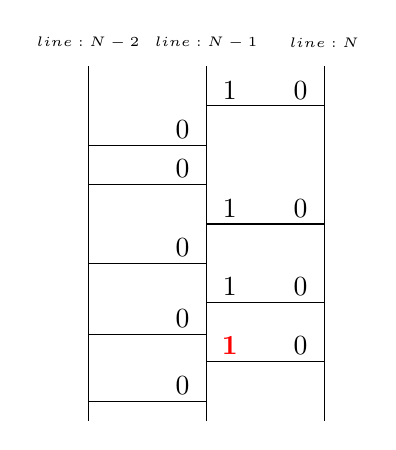
\begin{tikzpicture}
        \draw(0, -0.5) to (0, 4);
            \node at (0, 4.3){\tiny{$line:N-2$}};
            \draw(0, 3) to (1.5, 3);
                \node at (1.2, 3.2){$0$};
            \draw(0, 2.5) to (1.5, 2.5);
                \node at (1.2, 2.7){$0$};
            \draw(0, 1.5) to (1.5, 1.5);
                \node at (1.2, 1.7){$0$};
            \draw(0, 0.6) to (1.5, 0.6);
                 \node at (1.2, 0.8){$0$};
            \draw(0, -0.25) to (1.5, -0.25);
                \node at (1.2, -0.05){$0$};
        \draw(1.5, -0.5) to (1.5, 4);
            \node at (1.5, 4.3){\tiny{$line:N-1$}};
            \draw(1.5, 3.5) to (3, 3.5);
                \node at (1.8, 3.7){$1$};
                \node at (2.7, 3.7){$0$};
            \draw(1.5, 2) to (3, 2);
                \node at (1.8, 2.2){$1$};
                \node at (2.7, 2.2){$0$};
            \draw(1.5, 1) to (3, 1);
                \node at (1.8, 1.2){$1$};
                \node at (2.7, 1.2){$0$};
            \draw(1.5, 0.25) to (3, 0.25);
                \node at (1.8, 0.45){$\textcolor{red}{\textbf{1}}$};
                \node at (2.7, 0.45){$0$};

        \draw(3, -0.5) to (3, 4);
            \node at (3, 4.3){\tiny{$line:N$}};
    \end{tikzpicture}
    \caption{The line coding for $LC_{N-1}$ with imrpovement three is $101110$\underline{$0$}. The red, bold $1$ represents 
    the last left end point in $LC_{N-1}$, therefore the proceeding $0$ must be 
    included in $LC_{N-1}$. For every other $1$ in $LC_{N-1}$, a $0$ is omitted following 
    said $1$.}
    \label{fig:improvement3}
\end{figure}
\subsubsection{Combining All Three}
The combination of all three improvements can be done independently. 
Let $IC_{L(4,2,3,1)}$ be the \emph{improved line-based encoding} for $L_{(4,2,3,1)}$ 
by applying improvements 1-3 to $LC_{L(4,2,3,1)}$. Recall that $LC_{L}$ denotes the line-based encoding for some ladder $L$.
The $LC_{L(4,2,3,1)}$ for the ladder in Fig.\ref{fig:line-encoding} is $11\underline{0}10101\underline{0}0010101\underline{0}000$.
By applying imrpovement one, we get $11\underline{0}101011\underline{0}0010101\underline{0}$. 
Notice how the last three $0s$ from $LC_{L(4,2,3,1)}$ were removed because they represented $LC_{N}$.
By applying imrpovement two to improvememt one we get $11\underline{0}10011\underline{0}001001\underline{0}$.
Notice how the second, and eigth $1$ were removed because they are implied by 
the successive $0s$. By applying improvement three to the result of improvement 
two we get $11\underline{0}10011\underline{0}00101\underline{0}$. Notice how the last $0$ 
was removed from improvement two. This is because the $0$ is implied in $LC_{N-1}$
due to the configuration between of bars connecting lines $N-1$ and line $N$. The $IC_{L_(4,2,3,1)}$ for the ladder in Fig.\ref{Fig:allthree} 
is $IC_{L_(4,2,3,1)}=11\underline{0}10011\underline{0}00101\underline{0}$.\pagebreak

\begin{figure}[!htp]
     \centering
    \begin{tikzpicture}
         \draw(0, 0) to (0, 4);
             \node at (0, 4.3){\tiny{$line:N-3$}};
             \draw(0, 3.5) to (1.5, 3.5);
             \draw(0, 2.5) to (1.5, 2.5);
         \draw(1.5, 0) to (1.5, 4);
             \node at (1.5, 4.3){\tiny{$line:N-2$}};
             \draw(1.5, 3) to (3, 3);
             \draw(1.5, 3.8) to (3, 3.8);
             \draw(1.5, 2) to (3, 2);
             \draw(1.5, 1) to (3, 1);
         \draw(3, 0) to (3, 4);
             \node at(3, 4.3){\tiny{$line:N-1$}};
             \draw(3, 2.5) to (4.5, 2.5);
             \draw(3, 1.5) to (4.5, 1.5);
             \draw(3, 0.5) to (4.5, 0.5);
         \draw(4.5, 0) to (4.5, 4);
             \node at(4.5, 4.3){\tiny{$line:N$}};
     \end{tikzpicture}
     \caption{A ladder used to illustrate all three improvements $IC_{L}$. $IC_{L}=11\underline{0}10011\underline{0}00101\underline{0}$}
     \label{Fig:allthree}
\end{figure}